%\documentclass[referee]{aa} % for a referee version
\documentclass[onecolumn]{aa} % for a paper on 1 column  
%\documentclass[longauth]{aa} % for the long lists of affiliations 
%\documentclass[letter]{aa} % for the letters 
%\documentclass[bibyear]{aa} % if the references are not structured 
%                              according to the author-year natbib style
%\documentclass{aa}  


\usepackage{graphicx}
\usepackage{amsmath}
\usepackage{txfonts}

\begin{document} 


\title{Towards a Planckian standard kilogram}
\subtitle{}

\author{Michael Ebersold\thanks{michael.ebersold@uzh.ch}%\inst{1}
        \and
        Prasenjit Saha%\inst{2}\fnmsep
       }

\institute{Physik-Institut, University of Zurich, Winterthurerstrasse
  190, 8057 Zurich, Switzerland}

\date{}

\abstract
% context heading (optional)
% {} leave it empty if necessary  
{As the kilogram assumes its new definition in terms of $h,c,$ and the
  standard second, it is interesting to think about a possible future
  definition entirely in terms of fundamental constants.  A kilogram
  defined as an integer multiple of the Planck mass (or
  4594xxxx$\times\sqrt{\hbar c/G}$) would cause no significant change
  from its current value.}
% aims heading (mandatory)
{The practical hurdle to this Planckian kilogram is measuring $G$
  three or four orders of magnitude better than currently known, so as
  to find the unknown digits xxxx.  We study a possible scenario for
  doing so with an artificial two-body orbit.}
% methods heading (mandatory)
{The cleanest (admittedly, not the cheapest) option is to place the
  system on a Trojan orbit to minimize external gravitational
  perturbations, and enclose it in a cavity chilled to liquid-helium
  temperatures, to suppress radiation pressure.}
% results heading (mandatory)
{Data analysis would involve marginalizing over at least 15~nuisance
  parameters (6~for orbital parameters and 9~for fictitious forces)
  but that, we show, is feasible.}
% conclusions heading (optional), leave it empty if necessary 
{}

\keywords{}

\maketitle

\section{Introduction}

The reform of SI units to use quantum standards is an ongoing ``news
story'' in physics.\footnote{International Bureau of Weights and
  Measures, ``DRAFT 9th edition of the SI Brochure", BIPM.}  At the
heart of the reform are two quantum phenomena that appear on
macroscopic scales: the Josephson effect makes $h/e$ measurable as a
voltage-to-frequency ratio, while the quantum Hall effect makes
$h/e^2$ a standard resistance (the von~Klitzing constant).  These
enable electrical units to be defined in terms of $h$ and $e$.  A
further ingenious instrument, known as a watt balance, precisely
compares electrical and mechanical power, thus enabled mass to be
standardized in terms of $h$.  For a simple introduction to the new
SI, we refer the reader to the article on the ``LEGO watt
balance''.\citep{Chao15} The proposed redefinition of the kilogram is
an explicit value for $h$ and $c$, but we can think of it as
\begin{equation}
\mathrm{kg} \equiv 1.3563925\ldots \times 10^{50} \, \mathrm{s}^{-1}
                   \times \frac{h}{c^2}
\end{equation}
with the exact value to be decided.  As we can see, the kilogram is
coupled to the definition of a second.  That is not a problem in
practice, as the second is standardized orders of magnitude better
than any other unit.  Nonetheless, it is interesting to consider a
logical further step of decoupling the kilogram from other
definitions.  This could be done by introducing the gravitational
constant, since $\sqrt{hc/G}$ has dimensions of mass.
Historically, there have been several proposed unit systems that
included $G$ in some way,\cite{Tomilin1999} but the idea of including
both gravity and quantum mechanics in a unit system comes from
Planck.\cite{Planck99} In the process of working towards the radiation
law, Planck realized that $c,G,h$ and the Boltzmann constant $k_B$ (in
his notation $G\rightarrow f$, $h\rightarrow b$, $h/k_B\rightarrow a$)
naturally define units for mass, length, time, and temperature.
Indeed, Planck remarked that such units would be meaningful even in
non-human and extraterrestrial cultures.

A hypothetical Planckian SI unit system would have
\begin{equation} \label{eq:defs}
\begin{aligned}
\mathrm{kg} &= 4.594\ldots \times 10^7
               \left(\frac{\hbar c}{G}\right)^{\!1/2} \\
\mathrm{m}  &= 6.187\ldots \times 10^{34}
               \left(\frac{\hbar G}{c^3}\right)^{\!1/2} \\
\mathrm{s}  &= 1.854\ldots \times 10^{43}
               \left(\frac{\hbar G}{c^5}\right)^{\!1/2} \\
\mathrm{K}  &= 7.058\ldots \times 10^{-33}
               \left(\frac{\hbar c^5}{Gk_B^2}\right)^{\!1/2}
\end{aligned}
\end{equation}
with the numerical coefficients chosen so as to match the present
standards.  The square-rooted expressions are conventionally known as
the Planck mass, Planck length, and so on.  (They are actually
$\sqrt{2\pi}$ smaller than Planck's definitions.)  Extension to
electrical units is straightforward, but we will not discuss it here.
The Planck length, time, and temperature in themselves are extreme
scales, not probed by any known physical process, and presumably the
regime of quantum gravity.  But extreme scales do not harm if they are
only part of some expression, as they are here.  The Planck mass is
small but microscopically measurable: $\sim20\mu\mathrm{g}$.  This is
of the same order as the uncertainty in the prototype kilogram
itself.\footnote{\url{<https://www.bipm.org/utils/common/pdf/cms_m.pdf>}}
Hence the kilogram could be redefined as an integer multiple of the
Planck mass, without significantly perturbing its value.

The difficulty with Eq.~\eqref{eq:defs} is that all the expressions
involve $G$.  Given the current uncertainties in $G$,\cite{CODATA17}
Eq.~\eqref{eq:defs} would allow units to be standardized only to four
significant digits, which is obviously not enough.  Improvement by
several orders of magnitude would be needed, to make the Planckian
kilogram practicable.  In this paper, we study a scenario which may
make such an improvement possible.  The same process would suffice to
move the Kelvin scale to a Planckian basis as well.  A Planckian
second or metre, however, are not a prospect with anything like
present technology, because demands on the time standard are more
stringent still.

\begin{figure}
	\centering
	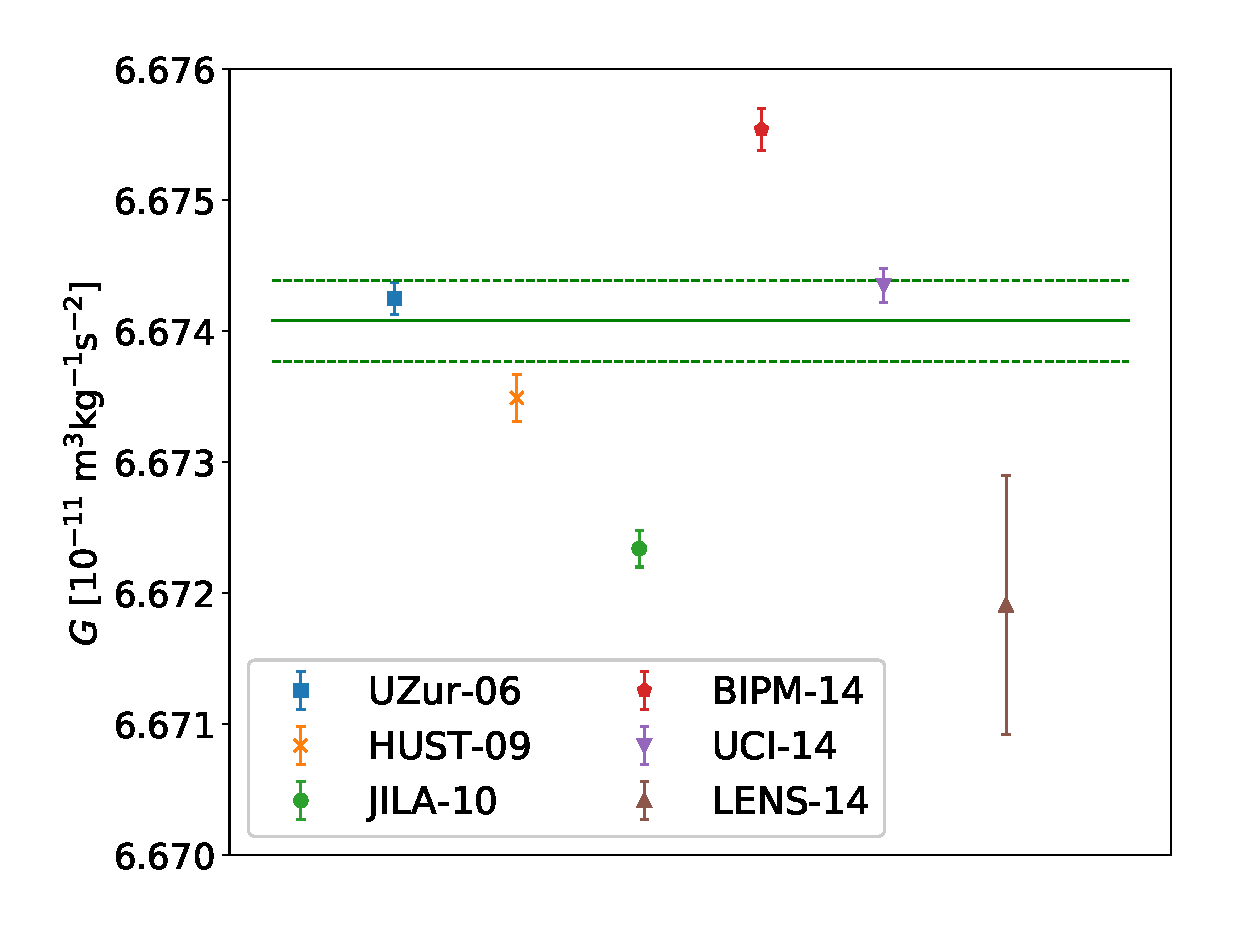
\includegraphics[width=\textwidth]{img/plotGmeas}
	\caption{Six of the most recent measurements of the gravitational constant $G$ with their uncertainties are plotted. The large disagreement is recognised immediately. The green lines represent the current recommended CODATA value and its uncertainty.\cite{CODATA17}}
	\label{fig:Gmeasurements}
\end{figure}

\section{A new approach to measure $G$}
In Fig.~\ref{fig:Gmeasurements} we plot the best-known recent
measurements of the gravitational constant. Three of them
(BIPM-14,\cite{Quinn14} UCI-14,\cite{Newman14} and
HUST-09\cite{Luo09}) were carried out using a torsion balance, whereas
UZur-06\cite{Schlamminger06} used a beam balance, and
JILA-10\cite{Parks10} measured the separation of two simple pendulums
in a gravitational field. They all tried to measure the very weak
gravitational force with a mechanical apparatus. The sixth measurement
(LENS-14\cite{Rosi14}) was performed with another approach, using cold
atom interferometry. Its uncertainty is a lot larger than the others,
but it could become more competitive in the future. However, a brief
glance on the plotted measurements shows the disagreement of current
$G$-values and suggests a demand for new, potentially different
techniques.  One remarkable idea is to use the helioseismic modes of
the Sun, because they depend on both the mass and $G$ times the mass
of the Sun,\cite{Ch-Dalsgaard05} but this strategy does not yet give
competitive accuracy in $G$.

\subsection{An artificial two-body gravitating system}
Newton's law of gravitation does not only explain why an apple falls
down from a tree, it also explains orbits. If one has two bodies of
masses $m_1$ and $m_2$, on which the only force acting is their
respective gravitational attraction, they will orbit around the common
center of mass, with the relative vector tracing an ellipse
described by Kepler's laws. The third law, relates the
orbital period $P$ to semimajor axis $a$ of the ellipse, as
\begin{equation}\label{eq:kepler3}
P^2 = \frac{4 \, \pi^2}{G(m_1+m_2)}a^3
\end{equation}
with the gravitational constant $G$ appearing in the proportionality
factor.  If one can measure the position of the two masses very
accurately and thus the orbit is known, it is possible to deduce the
gravitational constant.  So what we need is a freely-falling two-body
system. The only way to achieve this over some time, is to go into
space. Thus, one has to design a spacecraft with a cavity that
contains the two masses and a position measurement apparatus. The
cavity should shield the two-body system from environmental
influences. The spacecraft is then put in space, at a location where
tidal forces are minimal.  The stable Lagrange points of the Earth-Sun
system (that is, $L_4$ or $L_5$, also known as the Earth-Trojan
locations) would be suitable.

\begin{figure}
	\centering
	\includegraphics[width=0.9\textwidth]{img/sketchnonumb.pdf}
	\caption{Sketch on how the two masses inside the cavity of a spacecraft orbit around each other.}
	\label{fig:sketch}
\end{figure}

To get a feeling what the dimensions of such an experiment could be,
choose for example lead balls with a diameter of about 10~cm, their
mass then is about 6~kg. If one then chooses a semimajor axis of
15~cm, the orbital period would be roughly 3.5~hours and the
gravitational force acting between the two bodies is of order
$10^{-8}$~N.  In Fig.~\ref{fig:sketch} we show a sketch on how this
would look like. Treating this system with Newtonian gravity is justified, because corrections from general relativity would be of order $(v^2/c^2)$ and $(GM/rc^2)$, which for our two-body system are both very small numbers. To follow the mutual orbit of the two balls, best
would be a laser interferometry system, which can yield precisions
down to some nanometers.\cite{Loughridge13}

Such a system, if it could be set up, promises two advantages.  One is
the avoidance of any mechanical contact with the gravitating parts of
the experiment.  The other advantage lies in the behavior of signal
and noise.  The signal, which is essentially the distance travelled,
is proportional to time. The noise, however, would be almost
time-independent. This suggests that signal-to-noise would be
proportional to the length of the experiment, until it was limited by
systematic error. The achievable accuracy would therefore depend
entirely on how well external perturbations to the gravitational
two-body problem could be eliminated, or corrected for.  In following,
we consider the expected perturbations.

\subsection{Disturbing effects}

\textbf{Radiation pressure:} The envelope of the cavity needs to protect the two body-system from the constant bombardment of radiation and charged particles from the Sun. Since the activity of the Sun varies much, the spacecraft must be able to correct its position around the freely falling masses inside the cavity.\\
Furthermore, there is thermal radiation inside the cavity, that could disturb the orbit.
Using the Stefan-Boltzmann law, we can relate radiation pressure to the temperature inside the cavity. If we then specify to balls of diameter $d$, we can express the force on the balls as 
\begin{equation}
F = \frac{2 \pi^6 d^2 {k_\mathrm{B}}^4 T^4}{45 c^3 h^3}.
\end{equation}
As we can see, this force is highly temperature dependent. In order to minimize this influence, one should deploy a temperature as small as possible in the cavity. In fact, if a cooling system based on liquid helium is installed, temperature can be brought down to about 4 K. Such a low temperature results in a force on the balls in the order of $10^{-16}$~N. Compared to the gravitational force, this is orders of magnitude less and thus we don't have to worry about effects of radiation pressure.

\textbf{Influence of the position measurement:} 
The photons of the laser that measures the position of the two balls exert an additional force. If a laser with a power of 1~mW is used and not more than five measurements every second are performed, the force on the balls is in the same order as the influence of thermal radiation and thus negligible too.

\textbf{Coulomb force:}
Since the electromagnetic force is orders of magnitude stronger than the gravitational force, the balls must be absolutely neutral. A possible source of charges are cosmic rays or the solar wind, so the two bodies have to be adequately shielded by the enclosing shell.  If we want that the Coulomb force between the balls is in the same order as the effect of thermal radiation and thus negligible, the maximal allowed charge on the balls is about $6 \cdot 10^{-14}$~C, which corresponds to roughly $4 \cdot 10^5$ elementary charges.

\textbf{Coriolis effect:}
\label{sec:coriolis}
The Coriolis force is a fictitious force which only acts on moving bodies in a rotating reference frame. If we imagine the spacecraft located stationary at a Lagrange point of the Earth-Sun system, it is situated in a rotating frame around the Earth-Sun barycenter. Since the balls are moving with respect to this frame, there will be a Coriolis acceleration
\begin{equation}
\label{eq:coriolis}
\ddot{\vec{r}}_\mathrm{c} = - 2 \; \vec{\omega} \times \dot{\vec{r}}.
\end{equation}
In this formula, $\vec{\omega}$ is the angular velocity vector of the rotating frame and $\dot{\vec{r}}$ is the velocity vector in the two-body system.

\textbf{Centrifugal and tidal forces:}
\label{sec:tidal}
The free fall condition is not possible to achieve for both masses simultaneously since we are in a non-inertial, rotating frame and therefore have to account for centrifugal forces. The centrifugal acceleration $\ddot{\vec{r}}_{\mathrm{Z}}$ is proportional to the distance vector $\vec{r}$ and scales with $\omega^2$, where $\omega$ is the angular velocity of the Sun-Earth reference frame:
\begin{equation}
\label{eq:centrifugalacc}
\ddot{\vec{r}}_{\mathrm{Z}} = \vec{\omega} \times \left( \vec{\omega} \times \vec{r} \right) 
\end{equation}
In addition, there are tidal forces. If one mass is closer to the Sun, the gravitational force on it is slightly bigger than on the other mass. This results in a force perturbation, which is also proportional to $r$. One can approximate the tidal acceleration as
\begin{equation}
\label{eq:tidalacc}
\ddot{\vec{r}}_{\mathrm{\tau}} \approx \frac{2 \, G \, M_\odot}{R^3} \, \vec{r}.
\end{equation}
In this equation $M_\odot$ is the solar mass and $R$ is the radius of the orbit around the Sun. With Kepler's third law one can rewrite the tidal acceleration as a function of the orbital period squared of the Sun-Earth reference frame. Thus it scales the same way as the centrifugal force. To estimate the magnitude of the centrifugal and tidal acceleration relative to the gravitational acceleration between the two balls, we find that their ratio is proportional to the orbital periods squared
\begin{equation}\label{a_ratio}
\frac{\ddot{r}_{\mathrm{\tau}}}{\ddot{r}_\mathrm{G}} \propto \frac{P^2}{{P_\odot}^2} \approx 10^{-7},
\end{equation}
where $P_\odot$ corresponds to one year, whereas $P$ is the orbital period of the two balls. So tidal and centrifugal effects are about $10^{-7}$ times smaller than the respective gravity of the two balls.

\textbf{Gravitational field:}
Much attention has to be paid to the effect of the gravitational field of the spacecraft itself and the measurement apparatus. This certainly can't be neglected, but with a clever design, its effects can be minimized. For example an almost spherically symmetric spacecraft would probably be a good choice. It should also be possible to calculate the gravitational field caused by the components of the spacecraft at the positions of the balls. Then one can correct the equation of motion by adding an extra term that is accounting for the gravitational field. \\
A source of an additional gravitational field is Earth's moon and the other planets in the solar system. Fortunately, for this we don't need to correct if the whole system, consisting of the spacecraft and the two-body system, is moving through space together. Although, the spacecraft should be able to correct its position around the two balls to avoid a collision.


\section{Extracting $G$ from position measurement data}

In this section we will show how the gravitational constant can be
recovered from the position data of the two balls that the laser
interferometry measurement would provide.  But first we have to find
the orbital equation of motion for the two balls.

\subsection{Orbital equation of motion}
From Newtonian dynamics the equation of motion for a clean two-body system is given by 
\begin{equation}
\label{eq:eomeasy}
\ddot{\vec{r}} = - \frac{G M\, \vec{r}}{r^3}.
\end{equation}
Here $M$ denotes the sum of the masses $m_1$ and $m_2$, $G$ is the
gravitational constant and $r$ is the relative distance between the
two bodies. For simplicity we will abbreviate the product of $GM$ with
$k$.  Since our two-body system is in a rotating frame, we have to add
the term developed before for the Coriolis acceleration, as well as a
correction term for centrifugal and tidal forces. The latter can be
written with a constant symmetric $3 \times 3$ matrix $C$ as follows
\begin{equation}
\label{eq:tidal}
\ddot{\vec{r}}_{\mathrm{C}} = C \cdot \vec{r},
\end{equation}
or in terms of the individual components 
\begin{equation}
\label{eq:tidacom}
\left(\ddot{r}_\mathrm{C}\right)_i = \sum_{k=1}^{3} C_{ik} \: r_k.
\end{equation}
The reference frame is chosen such that the barycenter of the two-body
system is freely falling and has no tidal or fictitious forces acting
on it.  The balls, however, do experience such forces, because they
are not at the centre of mass.  The $C$ term can be thought of as a
first-order expansion of these forces.  So the full equation of motion
for the two balls looks as follows:
\begin{equation}
\label{eq:eom}
\ddot{\vec{r}} = - \frac{k\,\vec{r}}{r^3} - 2 \; \vec{\omega} \times \dot{\vec{r}} + C \cdot \vec{r}
\end{equation}

These are actually three coupled equations of motion, one for each spatial coordinate. Since all are second order differential equations, we need to give six initial conditions to determine the orbit.\\
We choose our coordinate system such that the orbital plane of the two-body system is in the $x-y$ plane. $\vec{\omega}$ is a constant vector that points in the direction of the rotation axis of the Earth-Sun reference frame. We will fit for $\vec{\omega}$, so we don't have to know it exactly before, but it can be estimated well and thus provides good starting points for the fit. The same is valid for the six components of the matrix $C$.
We choose our coordinate system such that the orbital plane of the two-body system is in the $x-y$ plane. $\vec{\omega}$ is a constant vector that points in the direction of the rotation axis of the Earth-Sun reference frame. We will fit for $\vec{\omega}$, so we don't have to know it exactly before, but it can be estimated well and thus provides good starting points for the fit. The same is valid for the six components of the matrix $C$.

Counting all unknown parameters in the equation of motion, we get
16. They correspond to 6 initial conditions, 6 components of the
matrix $C$, 3 components of the vector $\vec{\omega}$ and the object
of main interest, $k$, which contains the gravitational constant ($k =
GM$). Fitting for so many parameters is not an easy task, but it
should be possible because the parameters are approximately known in
advance.

\subsection{Markov Chain Monte-Carlo fit}

To fit for $k$ and the 15 accompanying nuisance parameters, we suggest
using a Markov Chain Monte-Carlo (MCMC) method, which are widely used
for similarly large parameter spaces.  MCMC is a Bayesian approach,
which uses the information provided by observed data about a set of
parameters, to update a prior state of knowledge/ignorance about the
set of parameters to become a posterior state of knowledge/ignorance
about a set of parameters. We will not describe in detail how MCMC
works, but refer the reader to an online tutorial from ESO
PyCoffee\footnote{\url{<http://eso-python.github.io/ESOPythonTutorials/ESOPythonDemoDay8_MCMC_with_emcee.html>}}
or an introduction paper from van
Ravenzwaaij et al.\cite{vanRavenzwaaij16}

We now briefly explain in what range the values of the parameters are
estimated.  Numbers are given in Table~\ref{tab:parameters}.  For the
parameter $k$, which is the product of the gravitational constant $G$
and the total mass $M$ we look at the current measured values for the
gravitational constant in Fig.~\ref{fig:Gmeasurements}, it is
reasonable to constrain its numerical value in SI units to values
between $6.671 \cdot 10^{-11}$ and $6.676 \cdot 10^{-11}$. The masses
of the two balls will not contribute to a larger uncertainty in $k$,
we choose them to be 6~kg.  The vector $\vec{\omega}$ accounts for the
rotation of the reference frame. If we say that the orbit of the balls
lies in the same plane as the orbital plane of the Earth,
$\vec{\omega}$ will point in $z$-direction with $x$ and $y$
components small. Thus $\omega_z$ is associated with the period
$P_\odot$ of one year through $2\pi/P_\odot$. Because the rotation
axis are conceivably not exactly aligned, we add some uncertainty. As
mentioned before, the $x$ and $y$ components are small, that is to
say, near zero in roughly the range of the uncertainty in
$\omega_z$.


The main contribution to the tidal term goes with $\omega^2$ and lies in the orbital plane. We are free to choose the $x$ and $y$ axis, so we choose it such that the $\omega^2$-contribution is in $x$-direction. The other five components then should be smaller, but we give some extra range to account for possible other perturbations.
The initial values for the positions can be guessed very accurately, since they are directly measured precisely. The initial velocity can be calculated easily and matched to the initial positions, therefore also yielding narrow parameter ranges.

\begin{table}%[ht]
	\centering
	\caption{This table shows the ranges in which the parameters numerical values in SI units are estimated to make sense and the value which was chosen to generate data.}
%	\begin{ruledtabular}
		\begin{tabular}{l c c}
			% The codes above determine the horizontal alignment in each column.
			% Options are l (left), r (right), c (centered), and p (paragraph).
			% The p option allows an entry to be broken into multiple lines, and
			% therefore requires a width specification, in this case 5 centimeters.
			parameter & range & chosen value \\
			\hline	% horizontal line to separate headings from data
			$k$ & $(8.0052$--$8.0112) \cdot 10^{-10}$ & $8.0088 \cdot 10^{-10}$ \\
			$\omega_x$ & $\pm 1.0 \cdot 10^{-8}$ & $0.02 \cdot 10^{-8}$ \\
			$\omega_y$ & $\pm 1.0 \cdot 10^{-8}$ & $-0.03 \cdot 10^{-8}$ \\
			$\omega_z$ & $(1.95$--$2.05) \cdot 10^{-7}$ & $1.996 \cdot 10^{-7}$ \\
			$C_{xx}$ & $0$--$5.0 \cdot 10^{-14}$ & $3.8 \cdot 10^{-14}$ \\
			$C_{yy}$ & $\pm 10^{-14}$ & $0.3 \cdot 10^{-14}$ \\
			$C_{zz}$ & $\pm 10^{-14}$ & $-0.2 \cdot 10^{-14}$ \\
			$C_{xy} = C_{yx}$ & $\pm 10^{-14}$ & $0.3 \cdot 10^{-14}$ \\
			$C_{yz} = C_{zy}$ & $\pm 10^{-14}$ & $0.1 \cdot 10^{-14}$ \\
			$C_{xz} = C_{zx}$ & $\pm 10^{-14}$ & $-0.4 \cdot 10^{-14}$ \\
			$x_0$ & $0.15 \pm 10^{-7}$ & $0.15$ \\
			$y_0$ & $\pm 10^{-7}$ & $0.0$ \\ 
			$z_0$ & $\pm 10^{-7}$ & $0.0$ \\ 
			$v_{x_0}$ & $\pm 10^{-7}$ & $0.0$ \\ 
			$v_{y_0}$ & ($7.30$--$7.31) \cdot 10^{-7}$ & $7.30698296 \cdot 10^{-5}$ \\
			$v_{z_0}$ & $\pm 10^{-7}$ & $0.0$ \\
		\end{tabular}
%	\end{ruledtabular}
	\label{tab:parameters}
\end{table}

In the next step, we set the parameters to a fixed ``true" value
within the range estimated. We have to keep in mind that $k$, $x_0$
and $v_{y_0}$ are linked together and there must not be contradictions
in the true values. The chosen values are displayed in the right
column of Table~\ref{tab:parameters}.  To simulate data we would
obtain from the position measurements, we integrate the equations of
motion. The time for one orbit without perturbations can be estimated
using Kepler's third law (\ref{eq:kepler3}). For the value of $k$
assumed above and a semi-major axis of $0.15$~m, this
results in an orbital period of roughly 12900 seconds or
3.5 hours. Here we integrate two orbits in 100000
steps, that would correspond to about 4 measurements per second,
which should be feasible. To the generated data, we add Gaussian noise
with a standard deviation of 10~nm. The value we use is just an estimate,
it would depend strongly on the measurement system that has been used.

\begin{figure}%[ht]
	\centering
	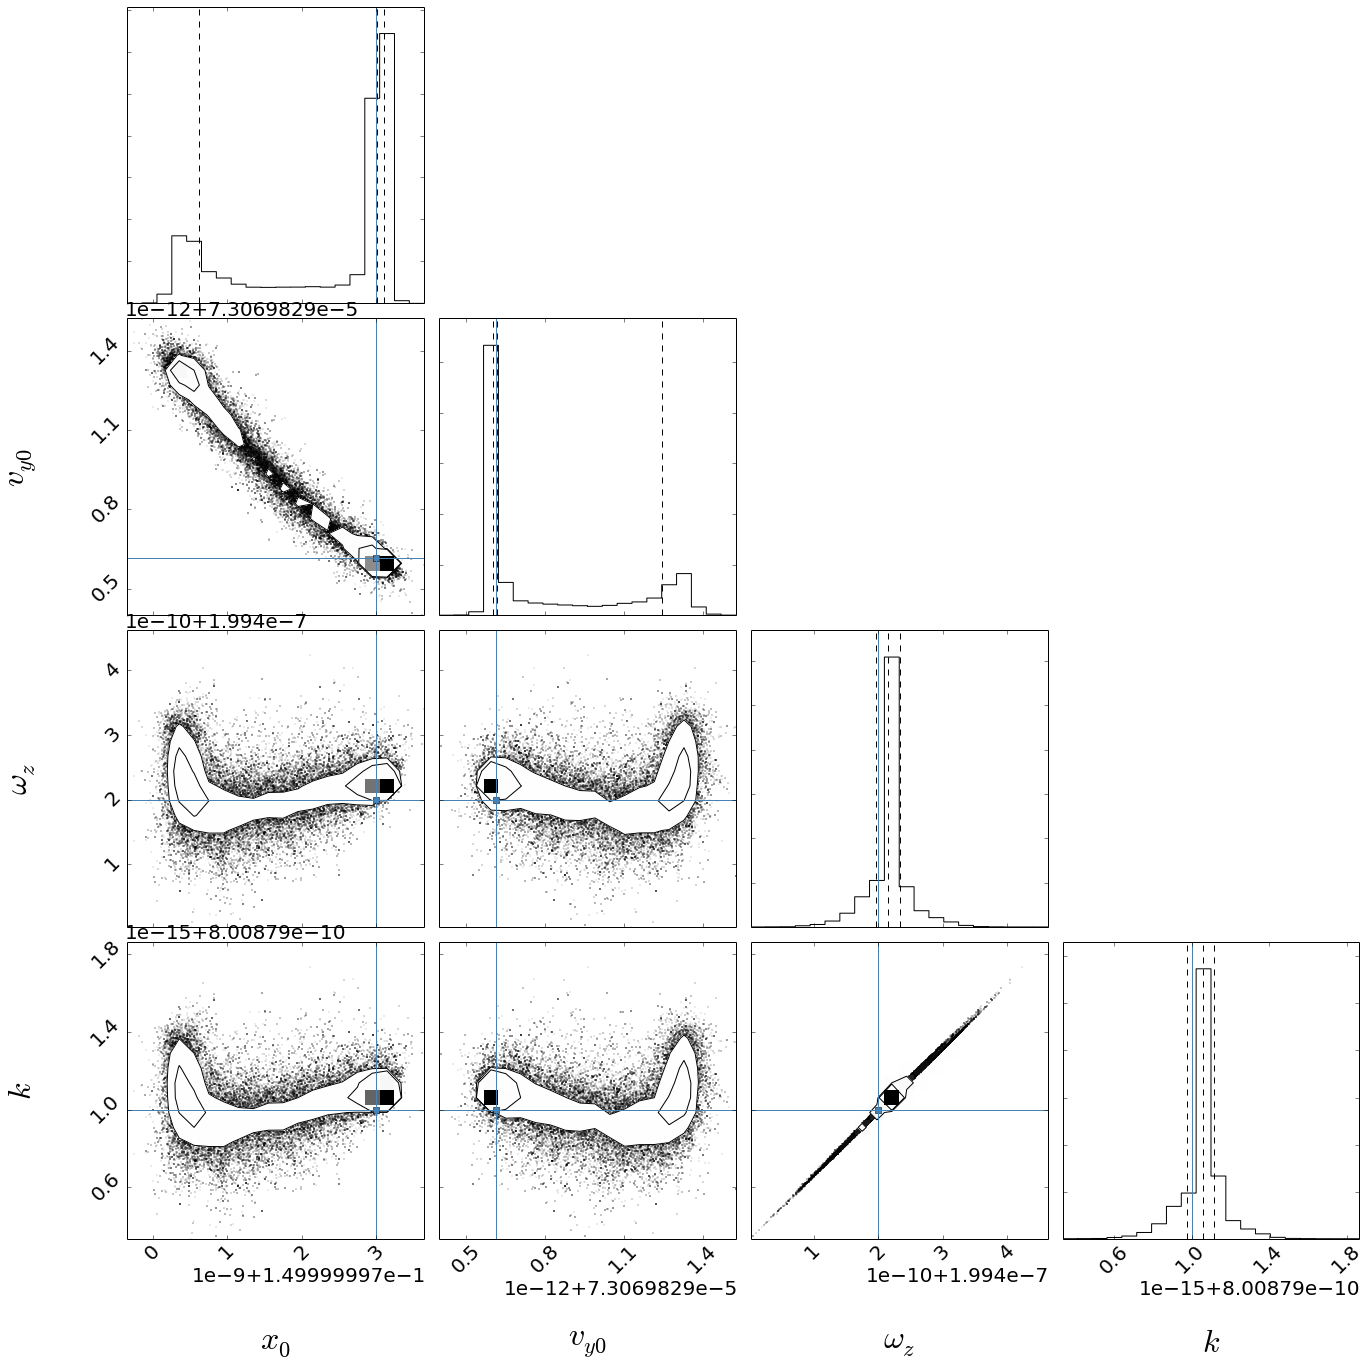
\includegraphics[width=1.0\textwidth]{img/4cornerfit.png}
	\caption{Corner plot of the posterior for 4 parameters: $x_0$, $v_{y_0}$, $\omega_z$ and $k$. Indicated with blue lines are the values we calculated the data from. The dashed lines in the histograms along the diagonal represent the median and the 0.16 and 0.84 percentiles respectively.}
	\label{fig:plotCorner4}
\end{figure}

A useful way to look at the samples of the posterior returned by the MCMC is to make a corner plot using a Python module named \textit{corner}.\cite{corner} The corner plot shows all the one- and two-dimensional projections of the posterior probability distributions and demonstrates quickly the covariances between parameters. Along the diagonal, the marginalized distribution for each parameter independently is shown.
In Fig.~\ref{fig:plotCorner4} an excerpt of the full corner plot is shown. 

To arrive at a best value with uncertainty for the gravitational constant, we take the mean and standard deviation of the marginalized distribution of the parameter $k$ and divide by the total mass of the balls. In this example the relative uncertainty of $k$ is roughly $10^{-7}$, so if the masses are measured to about the same precision, we can write for the gravitational constant $G$:
\begin{equation}\label{Gfit}
G = \left(6.674005 \pm 0.000001 \right) \cdot 10^{-11}  \frac{\mathrm{m}^3}{\mathrm{kg \, s}^2}
\end{equation}
This corresponds to a relative uncertainty of $1.5 \cdot 10^{-7}$ or 15 parts in a hundred million.

\section{Conclusion}
We have outlined an orbit experiment to measure the gravitational
constant $G$, and estimated the level of various disturbing effects
and how to correct for them.  Simulating the measurement process and
extraction of the gravitational constant indicates that $G$ could be
estimated to about $10^{-7}$ relative uncertainty.  This is about a
factor of 300 better than today's recommended CODATA value. A further increase in precision could be obtained by running the experiment longer. Measuring for 200 instead of two orbits could increase the precision by a factor of 10.
Hence, about the same relative uncertainty as for Planck's constant
$h$ ($1.2 \cdot 10^{-8}$)\cite{CODATA17} could be achieved. This then
would allow a future redefinition of the kilogram as an integer
multiple of the Planck mass.

We have not attempted in this paper to consider the cost of such an
experiment.  A mission to an Earth-Sun $L_4$ or $L_5$ with
liquid-helium cryogenics would obviously be very expensive, and also
carry an enhanced risk of unrepairable malfunctions killing the
experiment.  If the goals could be achieved in low-Earth orbit, the
prospects would be much more realistic.  The difficulty in low-Earth
orbit is that tidal acceleration due to the Earth would become
comparable to the two-body gravitational acceleration, with the Moon
and Sun also tidally perturbing the system.  The two-body system would
have a complicated orbit, very different from the nearly circular
orbit we have considered, and the initial conditions would have to be
chosen so as to avoid chaotic orbits.  Whether a sufficiently detailed
model for the tidal acceleration could be constructed and fitted to
the two-body orbital data is an open question.

\bibliographystyle{aa}
\bibliography{ms.bib}

\end{document}



bbibitem{BIPM16} International Bureau of Weights and Measures, ``DRAFT 9th edition of the SI Brochure", BIPM, (2016)

bbibitem{Chao15} L. S. Chao, S. Schlamminger, D. B. Newell, J. R. Pratt, F. Seifert, X. Zhang, G. Sineriz, M. Liu and D. Haddad, ``A LEGO Watt balance: An apparatus to determine a mass based on the new SI", \textit{American Journal of Physics}, 83:11:913--922 (2015).
% 2015AmJPh..83..913C

bbibitem{Tomilin1999} D. K. Tomilin, ``Natural Systems of Units. To the Centenary Anniversary of the Planck System,'' 
Proceedings of the XXII Workshop on high Energy Physics and field theory, 290 (1999).  

bbibitem{Planck99} M. Planck, ``\"{U}ber irreversible {S}trahlungsvorg\"{a}nge,'' 
Sitzungsberichte der K\"{o}niglich Preussischen Akademie der Wissenschaften zu Berlin, 479--480 (1899).  

bbibitem{BIPM} Bureau International des Poids et Mesures, Calibration and measurement services: Mass, \url{<https://www.bipm.org/utils/common/pdf/cms_m.pdf>}, (2015).

bbibitem{CODATA16} P. J. Mohr, D. B. Newell and B. N. Taylor, ``CODATA recommended values of the fundamental physical constants: 2014*, \textit{Reviews of Modern Physics}, 88(3):035009 (2016).

bbibitem{Quinn14} T. Quinn, C. Speake, H. Parks and R. Davis, ``The BIPM measurements of the Newtonian constant of gravitation $G$'', \textit{Philosophical Transactions of the Royal Society of London A: Mathematical, Physical and Engineering Sciences}, 372(2026) (2014).

bbibitem{Newman14} R. Newman, M. Bantel, E. Berg and W. Cross, ``A measurement of $G$ with a cryogenic torsion pendulum'', \textit{Philosophical Transactions of the Royal Society of London A: Mathematical, Physical and Engineering Sciences}, 372(2026) (2014).

bbibitem{Luo09} J. Luo, W. Liu, L. Tu, C. Shao, L. Liu, S. Yang, Q. Li and Y. Zhang, ``Determination of the Newtonian gravitational constant $G$ with time-of-swing method'', \textit{Phys. Rev. Lett.}, 102:240801 (2009).

bbibitem{Schlamminger06} S. Schlamminger, E. Holzschuh, W. Kündig, F. Nolting, R. E. Pixley, J. Schnurr and U. Straumann, ``Measurement of Newton's gravitational constant", \textit{Phys. Rev. D}, 74:082001 (2009).

bbibitem{Parks10} H. V. Parks and J. E. Faller, ``Simple pendulum determination of the gravitational constant", \textit{Phys. Rev. Lett.}, 105:110801 (2010).

bbibitem{Rosi14} G. Rosi, F. Sorrentino, L. Cacciapuoti, M. Prevedelli and G. M. Tino, ``Precision measurement of the Newtonian gravitational constant using cold atoms", \textit{Nature}, 510:518--521 (2014).

bbibitem{Ch-Dalsgaard05} J. Christensen-Dalsgaard, M.~P. Di Mauro,
  H. Schlattl and A. Weiss, ``On helioseismic tests of basic
  physics'', \textit{MNRAS}, 356:587--595 (2005).

bbibitem{Loughridge13} R. Loughridge and D. Y. Abramovitch, ``A tutorial on laser interferometry for precision measurements,'' 
American Control Conference, 3686--3703 (2013). 

bbibitem{esopycoffee} Fast and easy-to-implement Markov Chain Monte Carlo with the emcee package, ESO PyCoffee (2014),
\url{<http://eso-python.github.io/ESOPythonTutorials/ESOPythonDemoDay8_MCMC_with_emcee.html>}.

bbibitem{vanRavenzwaaij16} D. van Ravenzwaji, P. Cassey and S. D. Brown, ``A simple introduction to Markov Chain Monte-Carlo sampling,'' 
Psychonomic Bulletin {\&} Review, 1--12 (2016). 

bbibitem{corner} D. Foreman-Mackey, ``corner.py: Scatterplot matrices in Python,'' 
The Journal of Open Source Software (10), (2016).  



